\documentclass[
  UTF8,
  xcolor={dvipsnames,rgb},
  hyperref={colorlinks, citecolor=orange, linkcolor=black},
  aspectratio=169
  ]{beamer}

% \documentclass[
%   UTF8,
%   xcolor={dvipsnames,rgb},
%   hyperref={colorlinks, citecolor=orange, linkcolor=black},
%   ]{beamer}
\usepackage{xcolor}
\usepackage{appendixnumberbeamer}
\usepackage{bookmark}
\usepackage{ctex}
\usepackage{caption}
\usepackage{subfigure}
\usepackage{fontspec}
% \usepackage[english]{babel}
% \usepackage{csquotes}
\usepackage{amsmath}
\usepackage{amsthm}
\usepackage{unicode-math}
\usepackage{amssymb}
\usepackage{graphicx}
\usepackage{float}
\usepackage{color}
\usepackage[
    backend=biber,
    style=authoryear,
    sorting = nty,
    hyperref=true,
    doi=false
]{biblatex}

\setbeamerfont{footnote}{size=\tiny}

\usetheme[numbering=none]{Metropolis}

\usefonttheme{professionalfonts}
\setmainfont[Scale=1.0]{STIX Two Text}
\setsansfont[
    BoldFont={STIX Two Text SemiBold},
    ItalicFont={STIX Two Text Italic}
    ]{Arial}
\setmathfont{STIX Two Math}
\setCJKmainfont{KaiTi}[BoldFont=SimHei, ItalicFont=KaiTi]
\setCJKsansfont{KaiTi}[BoldFont=SimHei, ItalicFont=KaiTi]

\setbeamertemplate{caption}[numbered]
\setlength\bibitemsep{1.25\itemsep}

\setbeamertemplate{section in toc}[circle]
\setbeamertemplate{subsection in toc}[subsections numbered]
\setbeamertemplate{itemize item}[ball]
\setbeamertemplate{theorems}[ams style]
\setbeamertemplate{blocks}[rounded][shadow=true]
% \numberwithin{figure}{section}

\setbeamertemplate{footline}[frame number]

\theoremstyle{remark}
\newtheorem{assump}[theorem]{Identification Assumption}

\newenvironment{wideitemize}{\itemize\addtolength{\itemsep}{0.5em} }{\enditemize}
\addbibresource{./ref.bib}

\title{Taming the Factor Zoo (JoF 2020) 论文讲解}
\date{\today}
% multiple authors
\author{王悦 \and 蒋金骋 \and 董轩逸}
\institute{金融机器学习第一组}

\begin{document}

\begin{frame}
    \maketitle
\end{frame}

\begin{frame}
    \tableofcontents
\end{frame}

\section{概述}

\begin{frame}
    \frametitle{核心问题}

    \begin{wideitemize}
        \item 研究目标:已知因子池 \(h_{t}\),如何检验新加入因子 \(g_{t}\) 是否在横截面上对资产价格具有解释力?
        \item 存在的问题 \begin{enumerate}
            \item 检验哪个核心指标?
            \item \(h_{t}\) 中的因子已经很多,传统检验方法,如分组算收益率\parencite{FamaJournalofFinancialEconomics1993},GRS检验\parencite{GibbonsEconometrica1989},Fama-MacBeth回归\parencite{FamaJ.Polit.Econ.1973}等是否还适用?
            \item 计量上的问题:模型误设、遗漏变量,以及如何做推断
        \end{enumerate}
    \end{wideitemize}
\end{frame}

\begin{frame}
    \frametitle{本文的回应}
    \begin{enumerate}
        \item \textcite{Cochrane2009,CochraneTheJournalofFinance2011}建议检验因子对于随机贴现因子的载荷 (SDF loading) 的显著性,这一做法已经有文献采用\parencite{KozakTheJournalofFinance2018,KozakJournalofFinancialEconomics2020}
        \item 可能存在维数灾难的问题,需要对 \(h_{t}\) 进行变量筛选,使用 Double Selection LASSO\parencite{BelloniTheReviewofEconomicStudies2014}
        \item 用CV进行参数精调,采用DS策略选因子,理论推导渐进分布,构建``plug-in''方差估计量
    \end{enumerate}
\end{frame}

\begin{frame}
    \frametitle{本文的思路:Double Selection LASSO}

    \begin{wideitemize}
        \item 第三步 (检验新因子):将 \textcolor{red}{\(N\) 个资产收益时序上的平均值}对\textcolor{blue}{控制因子 \(h_{t} \in \mathcal{I}_1 \cup \mathcal{I}_2\) 和新因子 \(g_{t}\) 和资产在时序上的协方差}在\textcolor{orange}{截面上进行OLS回归},得到 \(g_{t}\) 的SDF loading
        \item 第一步 (选控制因子):将 \textcolor{red}{\(N\) 个资产收益时序上的平均值}对\textcolor{blue}{控制因子 \(h_{t}\) 和资产在时序上的协方差}进行LASSO回归,选出控制因子池 \(\mathcal{I}_1\)
        \item 第二步 (防止遗漏控制因子):将\textcolor{red}{控制因子 \(h_{t}\) 和资产在时序上的协方差}对\textcolor{blue}{新因子 \(g_{t}\) 和资产在时序上的协方差}进行LASSO回归,选出控制因子池 \(\mathcal{I}_2\)
        \item 得到第三步的估计量后,构建样本方差,做推断,判断新因子的解释能力
    \end{wideitemize}

\end{frame}

\begin{frame}
    \frametitle{本文的思路:Double Selection LASSO}

    \begin{figure}[H]
    \begin{center}
    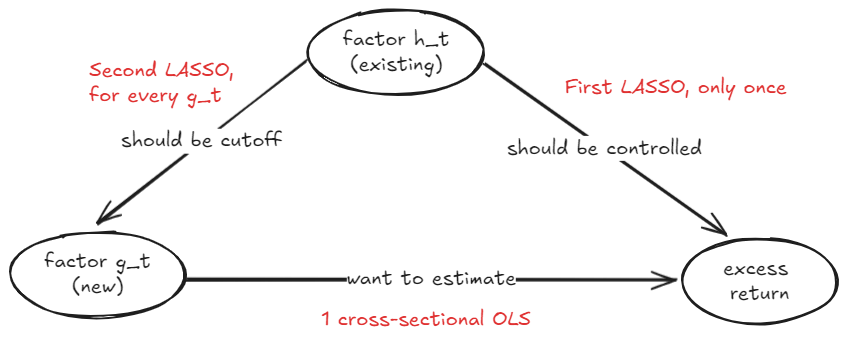
\includegraphics[width=0.8\textwidth]{../assets/idea.png}
    \end{center}
    \caption{研究思路}
    \label{pic:1}
    \end{figure}

\end{frame}

\section{计量模型}

\begin{frame}
    \frametitle{检验目标}
    如前所述,希望检验新因子的SDF loading,来判断其是否具有截面解释能力。这又分为两步,第一步,对每个资产在时间序列上计算其与因子的协方差,得到协方差矩阵 \(\hat{C}_g, \hat{C}_h\)
    \[
        \hat{C}_{g} \equiv  \begin{pmatrix}
        \mathrm{Cov}(r_{\cdot}^{1},g_{\cdot}^{1}) & \cdots & \mathrm{Cov}(r_{\cdot}^{1},g_{\cdot}^{d}) \\
        \vdots & \ddots & \vdots \\
        \mathrm{Cov}(r_{\cdot}^{N},g_{\cdot}^{1}) & \cdots & \mathrm{Cov}(r_{\cdot}^{N},g_{\cdot}^{d})
        \end{pmatrix}
    .\]
    其 \((i,j)\) 个元素可以理解为因子 \(g^{j}\) 在资产 \(i\) 上的风险暴露 (文中因子均指因子收益,如SMB)。
    \\
    \vspace{1em}
    第二步,用资产 \(i=1, \ldots ,N\) 的时序均值对风险暴露矩阵跑一个截面回归,得到SDF loading \(\lambda_g\),对其做统计检验。问题是控制因子 \(h\) 如何选择?
    \[\mathbb{E} \boldsymbol{r}_{i} =\iota \gamma_{0}+\hat{C}_{g}\lambda_{g}+\hat{C}_{h}\lambda_{h}+\boldsymbol{\epsilon}\]
\end{frame}

\begin{frame}
    \frametitle{因子选择:First LASSO}
    首先,必须要有控制因子,否则即使新因子是显著的,也无法将其解释作用与已有因子区分开来;其次,如果控制因子加的太多,会导致``维度诅咒''问题,模型拟合的效率会降低;如果漏掉了重要因子,即使估计量的渐进性质很好,在有限样本情况下也会有``模型误设''或者``正则化''的问题存在。
    \\
    \vspace{1em}
    因此,作者使用 Double Selection LASSO 来进行因子选择。分为两步,第一步是``筛出本就具有解释力的因子'',也就是跑一个截面的LASSO,在现有因子 \(h\) 中找到SDF loading非0的那些,加入控制集 \(\mathcal{I}_1\) 中

    \[( \hat{\lambda},\hat{\gamma} ) = \textrm{arg} \min_{\lambda,\gamma} \left\{ n^{-1} \Vert \bar{r}-\iota_{n}\gamma-\hat{C}_{h}\lambda \Vert^{2} + \tau_{0}n^{-1} \Vert \lambda \Vert_{1} \right\} .\]

\end{frame}

\begin{frame}
    \frametitle{因子选择:Second LASSO}
    第一步筛选中可能漏掉了一些因子,这些因子可能和SDF没有关系,但是\textcolor{red}{和新因子 \(g\) 有关}
    \begin{itemize}
        \item 后门准则,混淆因素,模型误设
        \item 作者的argument:这些因子可能具有非0的风险溢价,是遗漏变量;最坏的情况,即使这些因子是冗余的,将其加入也不会太影响模型的估计效率
    \end{itemize}
    第二步选择,用新因子池 \(g\) 中的每一个因子,对 \(h\) 中的所有因子跑一个截面LASSO (所以一共跑 \(d\) 个),将系数非0的那些 \(h\) 加入控制集 \(\mathcal{I}_2\) 中
    \[(\hat{\xi}_{i},\hat{\chi}_{j.}) = \textrm{arg} \min_{\xi_{j},\chi_{j.}} \left\{ n^{-1}\lVert \hat{C}_{g,.j}-\iota_{n}\xi_{j}-\hat{C}_{h}\chi_{j.}' \rVert^{2} + \tau_{1}n^{-1}\lVert \chi_{j.}' \rVert_{1}  \right\} , \; \forall j\]
\end{frame}

\begin{frame}
    \frametitle{第二步选择究竟在干什么}
    如果把这个LASSO看成一个OLS
    {\small
        \[
        \begin{pmatrix}
            \textcolor{red}{\mathrm{Cov}(r_{\cdot}^{1},g_{\cdot}^{1})} & \cdots & \mathrm{Cov}(r_{\cdot}^{1},g_{\cdot}^{d}) \\
            \vdots & \ddots & \vdots \\
            \textcolor{red}{\mathrm{Cov}(r_{\cdot}^{N},g_{\cdot}^{1})} & \cdots & \mathrm{Cov}(r_{\cdot}^{N},g_{\cdot}^{d})
            \end{pmatrix}=\mathbb{1}_{N\times d} \boldsymbol{\xi} + \begin{pmatrix}
            \mathrm{Cov}(r_{\cdot}^{1},h_{\cdot}^{1}) & \cdots & \mathrm{Cov}(r_{\cdot}^{1},h_{\cdot}^{d}) \\
            \vdots & \ddots & \vdots \\
            \mathrm{Cov}(r_{\cdot}^{N},h_{\cdot}^{1}) & \cdots & \mathrm{Cov}(r_{\cdot}^{N},h_{\cdot}^{d})
            \end{pmatrix}\times (\textcolor{red}{\chi_{1}},\dots,\chi_{d})
        \]
    }
    也就是说,对 \(h\) 中的因子而言,只要\textcolor{red}{其对资产的风险暴露}\textcolor{blue}{在截面上}与\textcolor{orange}{任何一个 \(g\) 中因子对资产的风险暴露}有相关性,就将其加入控制。
\end{frame}

\begin{frame}
    \frametitle{检验新因子}

    选出控制因子后,只需要再跑一个截面OLS
    \[
        \mathbb{E}\boldsymbol{r}_{i}=\iota \gamma_{0}+\hat{C}_{g}\lambda_{g}+\hat{C}_{h}\lambda_{h}+\boldsymbol{\epsilon}: \; \lambda_{h,j}=0, \; \forall j \notin \mathcal{I}_1 \cup \mathcal{I}_2
    \]
    然后检验哪些 \(\lambda_g\) 是显著非0的

\end{frame}

\begin{frame}
    \frametitle{统计推断}

    \begin{theorem}
        满足一系列条件的情况下,可以证明
        \[\sqrt{T}(\hat{\lambda}_g-\lambda_g) \xrightarrow{\mathcal{L}} \mathcal{N}_d (0,\Pi)\]
        并且,满足更多条件的情况下,可以构建估计量的样本方差 \(\hat{\Pi}\)
        \[\hat{\Pi} \xrightarrow{p} \Pi\]
    \end{theorem}
    这样就能做t检验了
\end{frame}

\begin{frame}
    \frametitle{方法总结}

    \begin{enumerate}
        \item 算因子和资产的风险暴露协方差矩阵 \(C_h,C_g\)
        \item 将 \(C_h\) 在截面上对资产均值回归,选出有效控制因子
        \item 将 \(C_g\) 在截面上对 \(C_h\) 回归,选出遗漏的控制因子
        \item 加入控制因子的 \(C_h\),将\(C_g\) 在截面上对资产均值回归,得到SDF loading,做t检验
    \end{enumerate}
\end{frame}

\section{实证步骤与结果}

\begin{frame}
    \frametitle{数据}
    
    \begin{wideitemize}
        \item 因子 \begin{itemize}
            \item 一共找了150个因子,来自Kenneth French的数据集,AQR数据集,以及一些因子论文作者的网站
            \item 用美国三大交易所的上市公司股票数据 (1976.7-2012.12),根据单因子分组,构建多空组合,算因子收益率
            \item 如果因子在2012年之前被提出,就是控制因子,否则是新因子
        \end{itemize}
        \item 资产 (投资组合) \begin{itemize}
            \item 用投资组合 (而非单只股票) 来算资产收益率
            \item 用150个因子中的连续因子,两两进行 \(3 \times 2\) 分组 (也就是每2个因子对应6个投资组合),去掉组内股票数小于10的那些因子组
            \item 一共得到750个投资组合,每个投资组合对应一个月度收益率序列
        \end{itemize}
    \end{wideitemize}
\end{frame}

\begin{frame}
    \frametitle{First LASSO}
    \[ \min_{\lambda,\gamma} \left\{ n^{-1} \Vert \bar{r}-\iota_{n}\gamma-\hat{C}_{h}\lambda \Vert^{2} + \textcolor{red}{\tau_{0}}n^{-1} \Vert \lambda \Vert_{1} \right\} .\]
    
    \begin{itemize}
        \item 基准情况下,选出了SMB,net external finance,change in shares outstanding 和 profit margin 这四个因子
        \item 注意 \(\tau_0\) 是一个超参数,会影响变量选择的结果
        \item 作者对其进行了稳健性检验,随机将样本时间段划分成10段,做200次
        \item 每一次,用10折交叉验证来确定 \(\tau_0\)
        \item 这样会得到200个不同的 \(\tau_0\),也就是200个不同的模型;从而每一次选出来的因子都不太一样,200个 \(\tau_0\) 的平均值用于基准模型
        \item 作者认为,如果单步LASSO是一个``对的''模型,那么应该有很少的几个因子每次都被选出来,剩下的因子永远不会被选出来
    \end{itemize}

\end{frame}

\begin{frame}

    \frametitle{First LASSO 结果}
    \begin{figure}[H]
    \begin{center}
    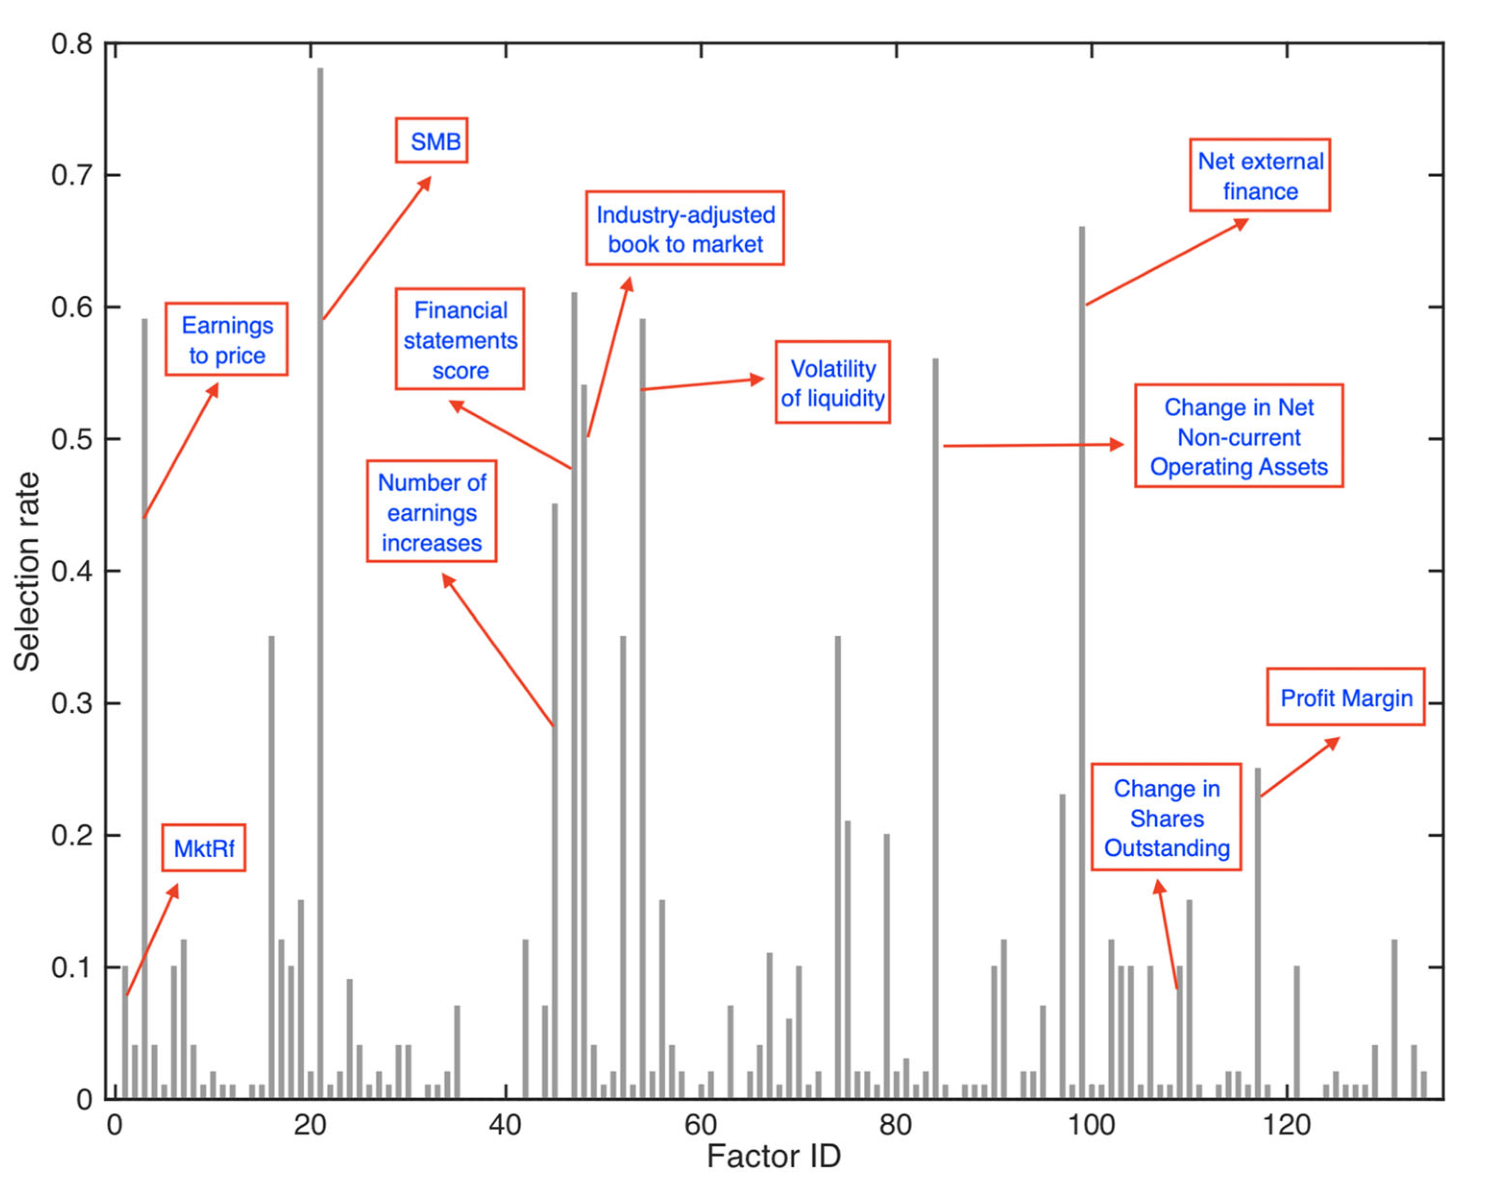
\includegraphics[width=0.55\textwidth]{../assets/stage1.png}
    \end{center}
    \caption{First LASSO 200次模拟结果}
    \label{pic:2}
    \end{figure}


\end{frame}


\begin{frame}
    \frametitle{Second LASSO}
    \[\min_{\xi_{j},\chi_{j.}} \left\{ n^{-1}\lVert \hat{C}_{g,.j}-\iota_{n}\xi_{j}-\hat{C}_{h}\chi_{j.}' \rVert^{2} + \textcolor{red}{\tau_{1}}n^{-1}\lVert \chi_{j.}' \rVert_{1}  \right\} , \; \forall j\]

    \vspace{1em}
    第二阶段选出了更多的因子,有20-80个,正文中并没有汇报具体是哪些;同样用200次CV取平均来确定超参数


\end{frame}

\begin{frame}
    \frametitle{DS Estimator 估计结果及比较}

    \begin{figure}[H]
    \begin{center}
    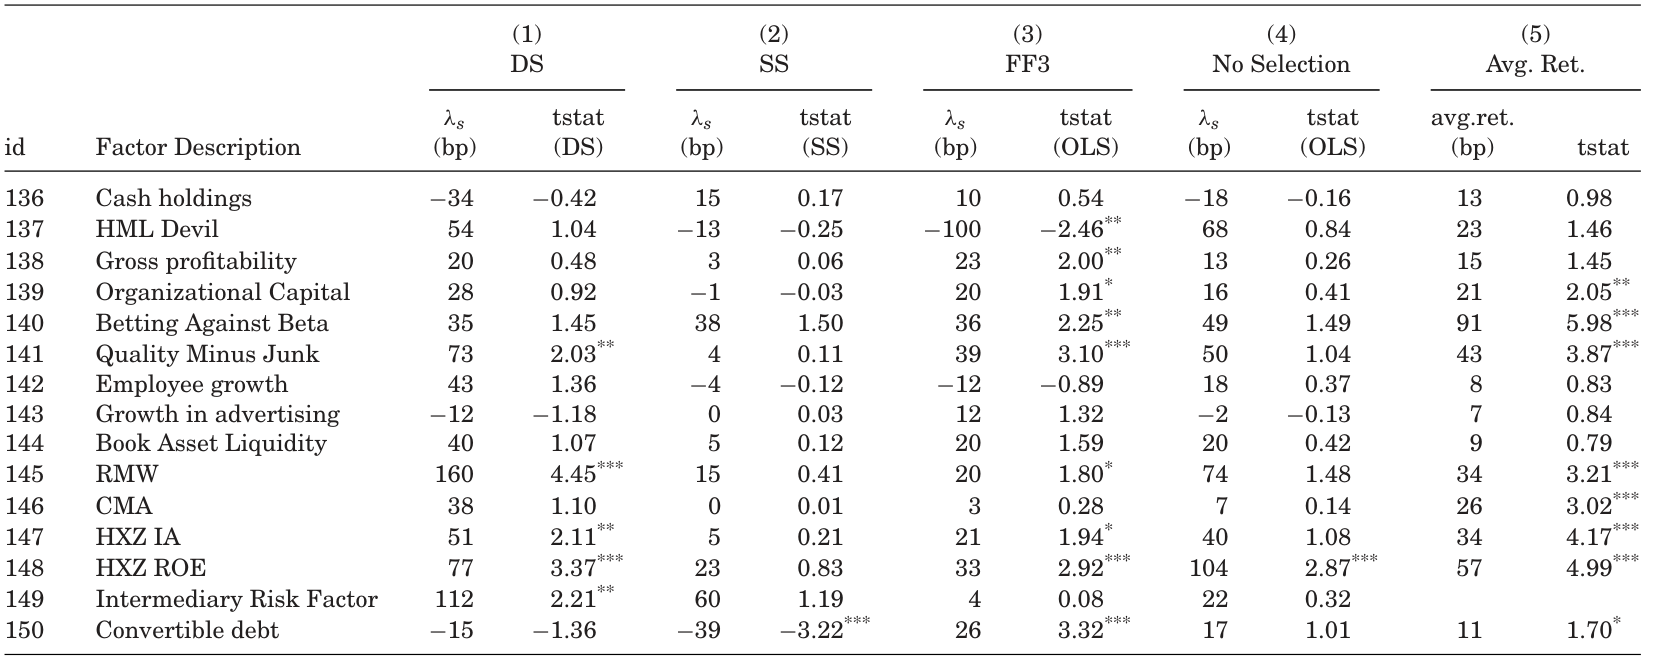
\includegraphics[width=0.8\textwidth]{../assets/DS.png}
    \end{center}
    \caption{不同方法因子选择结果}
    \label{pic:DS}
    \end{figure}
    前四列是控制变量 + SDF loading,第五列是 Fama-French 回归,估计系数用单位风险暴露做了标准化

\end{frame}

\begin{frame}
    \frametitle{递归检验}
    \begin{figure}[H]
    \begin{center}
    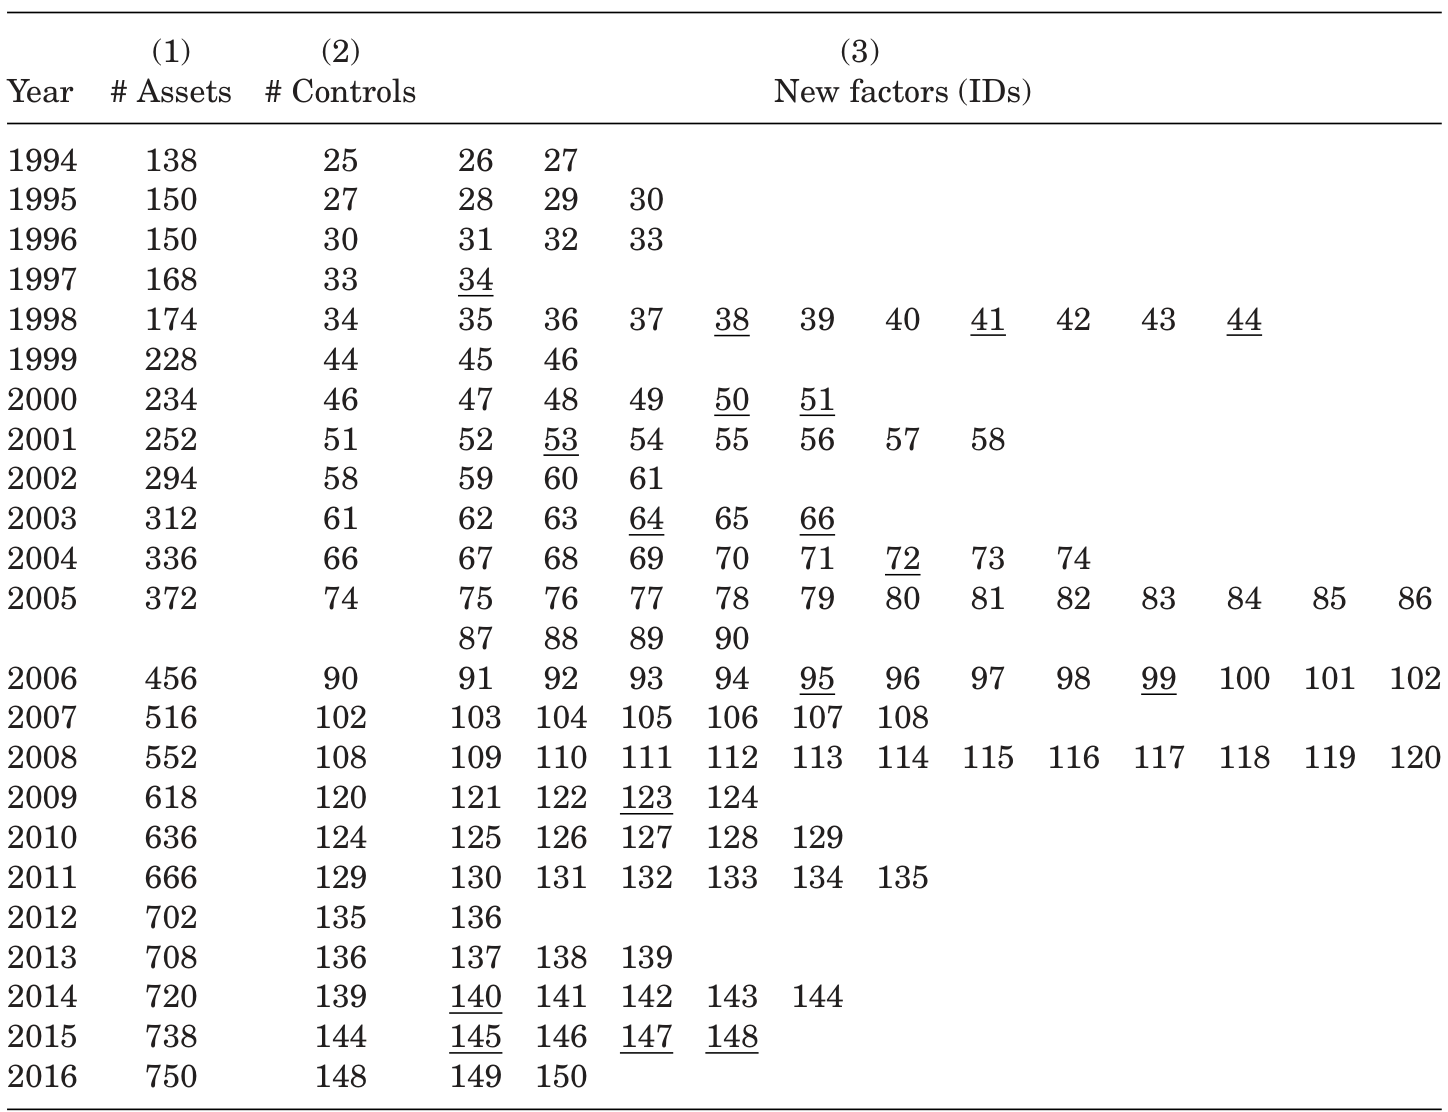
\includegraphics[width=0.45\textwidth]{../assets/recursive.png}
    \end{center}
    \caption{递归检验结果}
    \label{pic:recursive}
    \end{figure}
    
    从1994年开始,递归地使用DS LASSO对文献中提出的新因子进行检验;下划线代表显著

\end{frame}

\begin{frame}
    \frametitle{总结}

    \begin{wideitemize}
        \item 研究目的:检验新因子的横截面预测能力 \(\iff\) 检验SDF loading的显著性
        \item 需要控制已有因子 \(\implies\) 用LASSO选出已经具有预测能力的因子,作为控制变量
        \item (本文创新) LASSO可能存在遗漏变量和模型误设等缺陷 \(\implies\) 加入第二步LASSO,选择和新因子的风险暴露相关性较高的那些因子,加入控制变量中
        \item 结论 \begin{enumerate}
            \item 发现一些新因子具有解释力,与传统方法的结果差别较大
            \item DS LASSO 模型结果对于超参数比较稳健
            \item 递归检验仅确认了部分因子 (被提出时) 具有解释力
        \end{enumerate}
    \end{wideitemize}
\end{frame}

\appendix

\begin{frame}[allowframebreaks]
  \printbibliography
\end{frame}


\end{document}